\documentclass[14pt]{extarticle}
\usepackage{amsmath}
\usepackage{amssymb}
\usepackage{tikz}
%\usetikzlibrary{calc}
\usetikzlibrary{trees}
\usepackage{hyperref}
\usepackage{graphicx}
\graphicspath{ {../../chap08/} }
\usepackage[top=0.75in, bottom=0.75in, left=0.75in, right=0.75in]{geometry}
\newcommand*{\Scale}[2][4]{\scalebox{#1}{\ensuremath{#2}}}%
\usepackage[shortlabels]{enumitem}
\usepackage[most]{tcolorbox}
\definecolor{bg}{RGB}{255,249,227}
% \usepackage{showframe}
\title{\vspace{-5ex}Math 208 Section 8.4}
\date{\vspace{-10ex}}
\usepackage{multicol}
\setlength{\columnsep}{1cm}


\begin{document}
\maketitle		
\section*{Homework, Reading, and Other}
\begin{itemize}
	\item Section 8.1, 8.2
	\item Section 8.3
	\item Section 8.3
	\item Extra Credit - 2 points!\\
	Solve problem 8.3 number 61 for the general case of i rolls, where i = 1, 2, 3, 4, 5, 6, 7. (Hint: Think of factorials and combinations. See example 4 on page 413	(section 8.2))
\end{itemize}

\section{Goals}
\textbf{Bayes Formula}
\begin{align*}
	P(U_1|B) =
	\frac{\text{
			the product of the branch probabilities leading to B through $U_1$}}
	{\text{
			the sum of all branch products leading to B}}
\end{align*}

% Set the overall layout of the tree
\tikzstyle{level 1}=[level distance=3.5cm, sibling distance=3.5cm]
\tikzstyle{level 2}=[level distance=3.5cm, sibling distance=2cm]

% Define styles for bags and leafs
\tikzset{
	treenode/.style = {shape=rectangle, rounded corners,
		draw, align=center,
		%top color=white, bottom color=blue!20
	},
	payoff/.style    = {align=center, inner sep=0.1em, text width=1.5em},
	left side node/.style={above left, inner sep=0.1em},
	right side node/.style={above right, inner sep=0.1em}
}
\begin{tikzpicture}
	[
	grow                    = right,
	sibling distance        = 10em,
	level distance          = 4em,
	%	every node/.style       = {font=\footnotesize},
	sloped
	]
	\node [treenode] {Start}
	child{node [treenode] {$U_2$} 
		child{
			node [treenode] {B} edge from parent node[left side node] {}
		}
		child{
			node [treenode] {A} edge from parent node[left side node] {}
		}
		edge from parent node[right side node] {}
	}
	child{node [treenode] {$U_1$} 
		child{
			node [treenode] {B} edge from parent node[left side node] {}
		}
		child{
			node [treenode] {A} edge from parent node[left side node] {}
		}
		edge from parent node[right side node] {}
	};
\end{tikzpicture}

\section{8.4: Bayes Formula}
Previously we talked about conditional probability where we update our estimate of an event happening based upon some previous event having occurred. Today, we cover a similar case only now we ask what is the probability of a previous event having occurred knowing that we just measured an event.
\\\\
In other words knowing that B occurred, what is the probability that $U_1$ occurred?

\subsection{The Ball Example}
Recall drawing white and blue balls? Two balls are drawn in succession, without replacement, from a box containing 3 blue and 2 white balls. Note that $S=\{WW, WB, BW, BB\}$.
\\\\
\begin{tikzpicture}
	[
	grow                    = right,
	sibling distance        = 10em,
	level distance          = 4em,
	%	every node/.style       = {font=\footnotesize},
	sloped
	]
	\node [treenode] {Start}
	child{node [treenode] {$B_1$} 
		child{
			node [treenode] { $B_2\to \frac{3}{10}$} edge from parent node[right side node] {$2/4$}
		}
		child{
			node [treenode] { $W_2\to \frac{3}{10}$} edge from parent node[right side node] {$2/4$}
		}
		edge from parent node[right side node] {$3/5$}
	}
	child{node [treenode] {$W_1$} 
		child{
			node [treenode] {$B_2\to \frac{3}{10}$} edge from parent node[right side node] {$3/4$}
		}
		child{
			node [treenode] {$W_2\to \frac{1}{10}$} edge from parent node[right side node] {$1/4$}
		}
		edge from parent node[right side node] {$2/5$}
	};
\end{tikzpicture}
\\\\
Knowing that the second ball was white, what is the probability that the first ball was white? In other words, what is $P(W_1|W_2)$?
\\\\
From conditional probability, we have
$$P(W_1|W_2) = \frac{P(W_1 \cap W_2))}{P(W_2)}$$
From the tree diagram, we have
$$P(W_2)=P(W_1 \cap W_2) + P(W_1\cap B_1)$$
Combining and rearranging, we get
$$P(W_1|W_2) = \frac{P(B|W_1)P(W_1)}{P(B|W_1)P(W_1) + P(B|W_2)P(W_2)}$$
In words, which seems easier
\begin{align*}
	P(W_1|W_2) =
	\frac{\text{
			the product of the branch probabilities leading to $W_2$ through $W_1$}}
	{\text{
			the sum of all branch products leading to $W_2$}}
\end{align*}
For our example then,
$$P(W_1|W_2) = \frac{(2/5)(1/4)}{(2/5)(1/4) + (3/5)(1/2)} = \frac{1/10}{4/10} = \frac{1}{10}*\frac{10}{4}= 1/4$$


\subsection{Disjoint}
Looking at our tree, we see it is not possible to choose a white and blue ball on the first draw. This is very important. When calculating up the tree, the U we seek must be disjoint from the other U possibilities.
\\
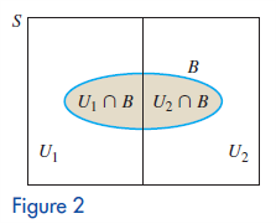
\includegraphics[width=0.4\linewidth]{partition2}
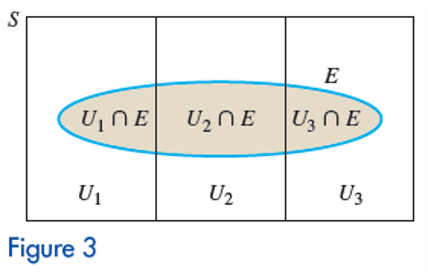
\includegraphics[width=0.5\linewidth]{partition3}
\\
\subsection{Bayes Formula}
\begin{tcolorbox}[enhanced jigsaw,colback=bg,boxrule=0pt,arc=0pt] 
	Let $U_1, U_2, \cdots, U_n$ be n mutually exclusive events. And let E be an arbitrary event. Then
	\begin{align*}
		P(U_1|E) = \frac{P(E|U_1)P(U_1)}{P(E|U_1)P(U_1) + P(E|U_2)P(U_2) + \cdots + P(E|U_n)P(U_n)}
	\end{align*}
	or
	$$P(U_1|E) =
	\frac{\text{
			the product of the branch probabilities leading to E through $U_1$}}
	{\text{
			the sum of all branch products leading to E}}$$
	This holds for all other disjoint $U_i$.
\end{tcolorbox}

\subsubsection{Example} 
\textbf{HW 61: Police Science}: A new lie-detector test has been devised and must be tested before it is used. One hundred people are selected at random, and each person draws a card from a box of 100 cards. Half the cards instruct the person to lie, and the others instruct the person to tell the truth. Of those who lied, 80\% fail the new lie-detector test (that is, the test indicates lying). Of those who told the truth, 5\% failed the test. What is the probability that a randomly chosen subject will have lied given that the subject failed the test? That the subject will not have lied given that the subject failed the test?
\\\\
Let L = Lie, T = Truth, P = Pass, F = Fail; then
\\\\

% Set the overall layout of the tree
\tikzstyle{level 1}=[level distance=4cm, sibling distance=4.0cm]
\tikzstyle{level 2}=[level distance=4cm, sibling distance=2cm]
% Define styles for bags and leafs
\tikzstyle{bag} = [text width=4em, text centered]
\tikzstyle{end} = [circle, minimum width=3pt,fill, inner sep=0pt]
\tikzset{
	treenode/.style = {shape=rectangle, rounded corners,
		draw, align=center,
		%top color=white, bottom color=blue!20
	},
	payoff/.style    = {align=center, inner sep=0.1em, text width=1.5em},
	left side node/.style={above left, inner sep=0.1em},
	right side node/.style={above right, inner sep=0.1em}
}

\begin{tikzpicture}
	[
	grow                    = right,
	sibling distance        = 10em,
	level distance          = 4em,
%	every node/.style       = {font=\footnotesize},
	sloped
	]
	\node [treenode] {Start}
		child{node [treenode] {L} 
		child{
			node [treenode] {$P\to .475$} edge from parent node[right side node] {$.95$}
		}
		child{
			node [treenode] {$F\to .025$} edge from parent node[right side node] {$.05$}
		}
		edge from parent node[right side node] {$1/2$}
	}
	child{node [treenode] {T} 
		child{
			node [treenode] {$P\to .1$} edge from parent node[right side node] {$.2$}
		}
		child{
			node [treenode] {$F\to .4$} edge from parent node[right side node] {$.8$}
		}
		edge from parent node[right side node] {$1/2$}
	};
\end{tikzpicture}
\\\\
$$\sum P = .4+.1+.025+.475 = 1$$
Answering the questions:
\begin{align*}
	P(L|F) &= \frac{.4}{.4+.025}= 0.9411 \\
	P(T|F) &= \frac{.025}{.425} = 0.0588
\end{align*}
Since lying and truth-saying are complements, we may also calculate this as $P(T|F) = 1 - P(L|F)$. Just be cautious with this shortcut.

\noindent\rule{\textwidth}{1pt}
{\footnotesize Copyright (C) 2021 Garold Dalton --- Released under GNU General Public License v3.0}


\cleardoublepage


\end{document}
